\clearpage
\section*{Appendix A: Spectra of the Six Channels in Each Repetition}

The Welch spectra were drawn with the same data and parameters as in Part~2. The dashed lines show the stimulation frequency and its multiples. The amplitude is in decibels relative to one unit of data squared per hertz.

\begin{figure}[p]
\centering
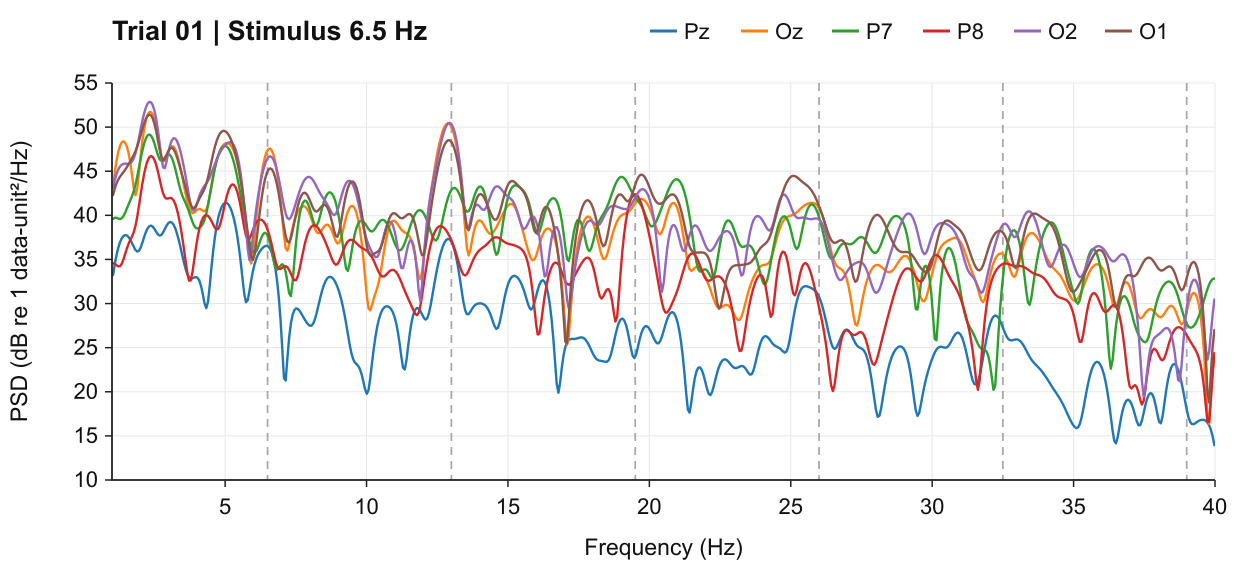
\includegraphics[width=0.9\textwidth,height=0.4\textheight,keepaspectratio]{fig15_ssvep_trial01_6p5hz.png}
\caption{Repetition 1 with a stimulation frequency of 6.5~Hz; all six channels are shown on one axis.}
\label{fig:app15}
\end{figure}

\begin{figure}[p]
\centering
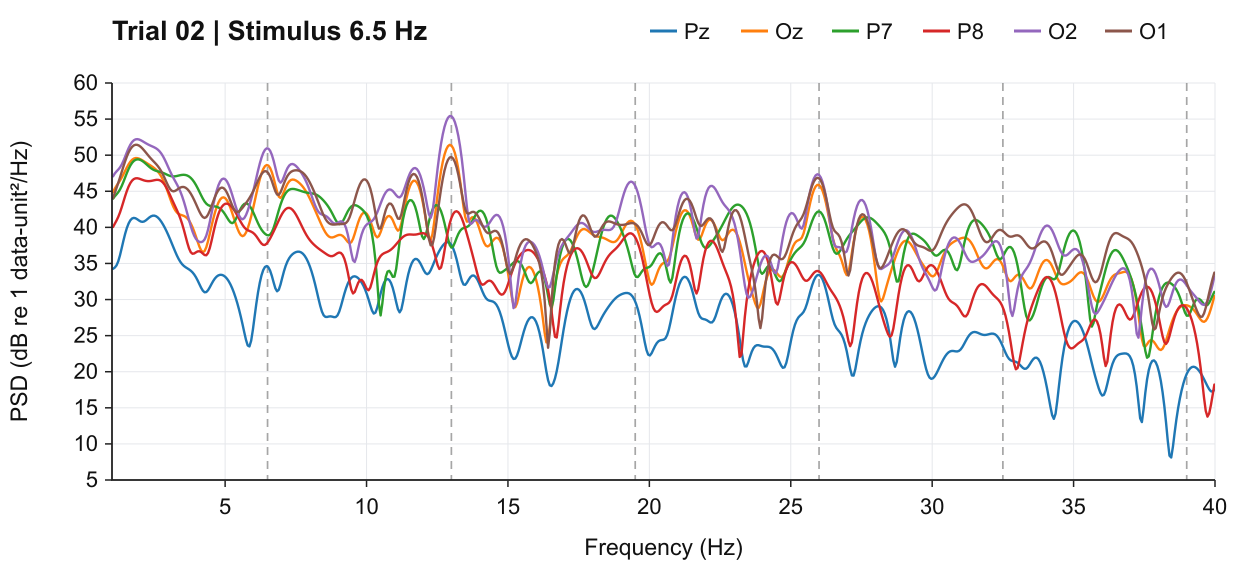
\includegraphics[width=0.9\textwidth,height=0.4\textheight,keepaspectratio]{fig16_ssvep_trial02_6p5hz.png}
\caption{Repetition 2 with a stimulation frequency of 6.5~Hz; all six channels are shown on one axis.}
\label{fig:app16}
\end{figure}

\begin{figure}[p]
\centering
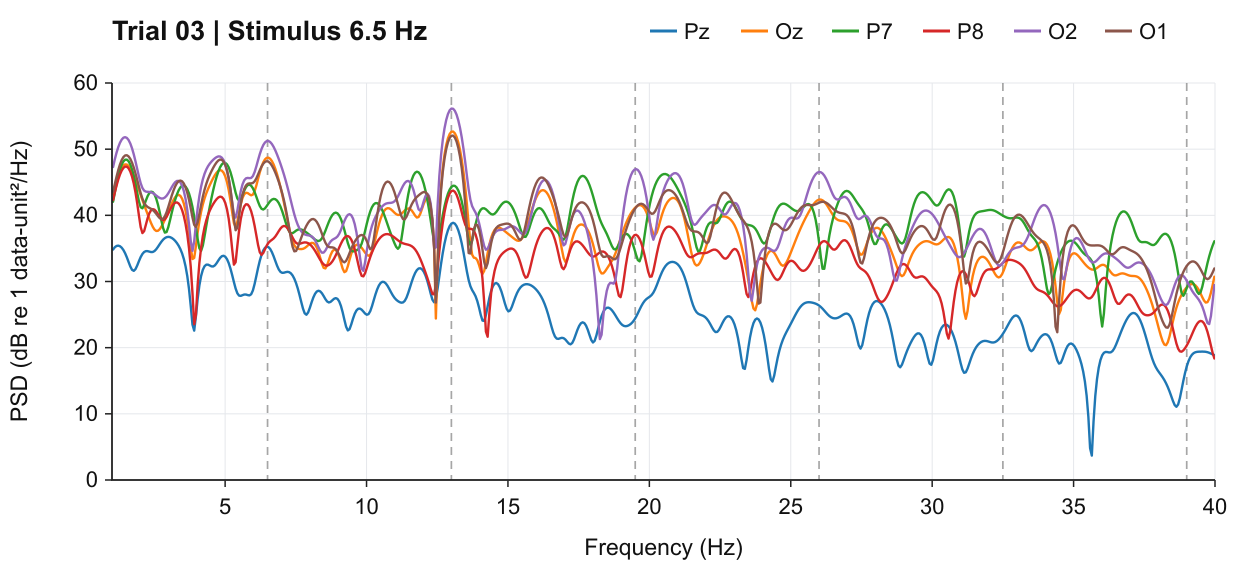
\includegraphics[width=0.9\textwidth,height=0.4\textheight,keepaspectratio]{fig17_ssvep_trial03_6p5hz.png}
\caption{Repetition 3 with a stimulation frequency of 6.5~Hz; all six channels are shown on one axis.}
\label{fig:app17}
\end{figure}

\begin{figure}[p]
\centering
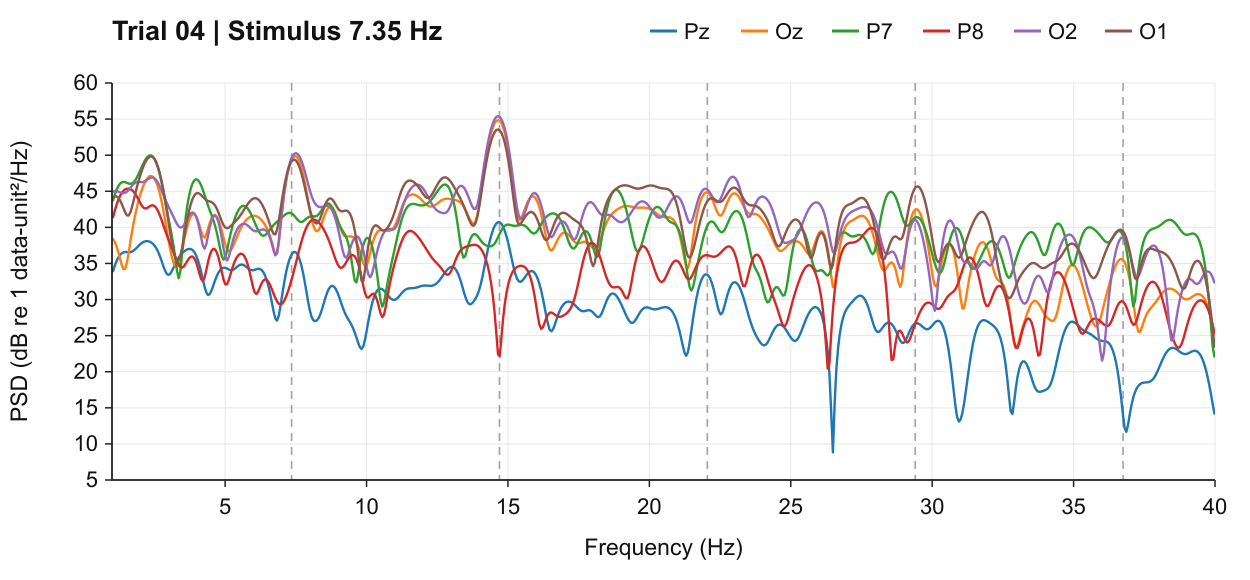
\includegraphics[width=0.9\textwidth,height=0.4\textheight,keepaspectratio]{fig18_ssvep_trial04_7p35hz.png}
\caption{Repetition 4 with a stimulation frequency of 7.35~Hz; all six channels are shown on one axis.}
\label{fig:app18}
\end{figure}

\begin{figure}[p]
\centering
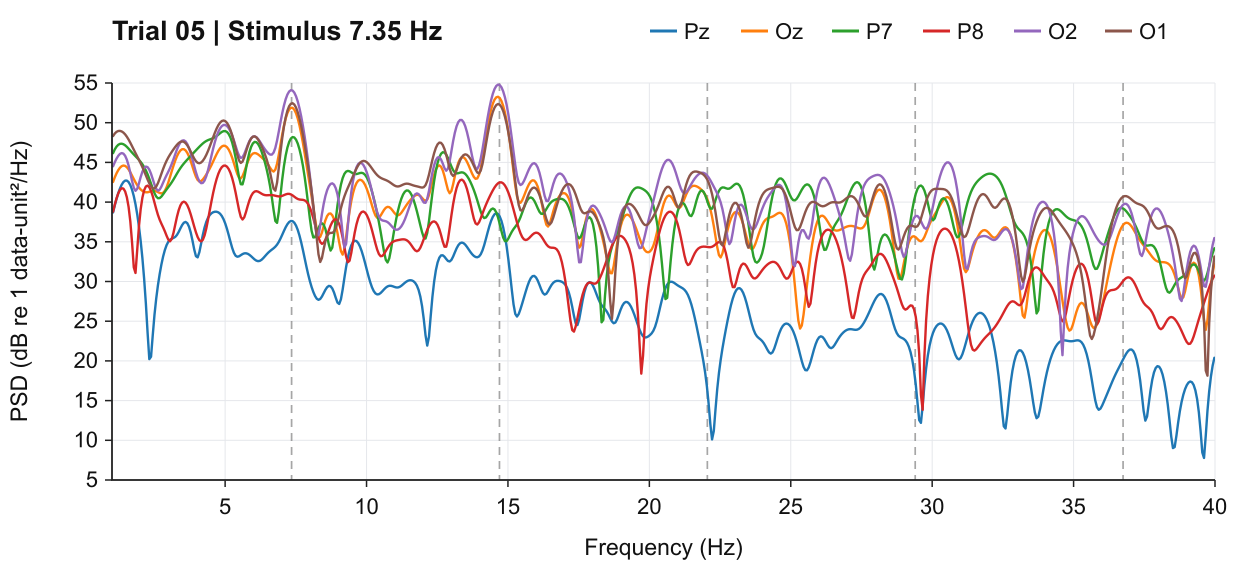
\includegraphics[width=0.9\textwidth,height=0.4\textheight,keepaspectratio]{fig19_ssvep_trial05_7p35hz.png}
\caption{Repetition 5 with a stimulation frequency of 7.35~Hz; all six channels are shown on one axis.}
\label{fig:app19}
\end{figure}

\begin{figure}[p]
\centering
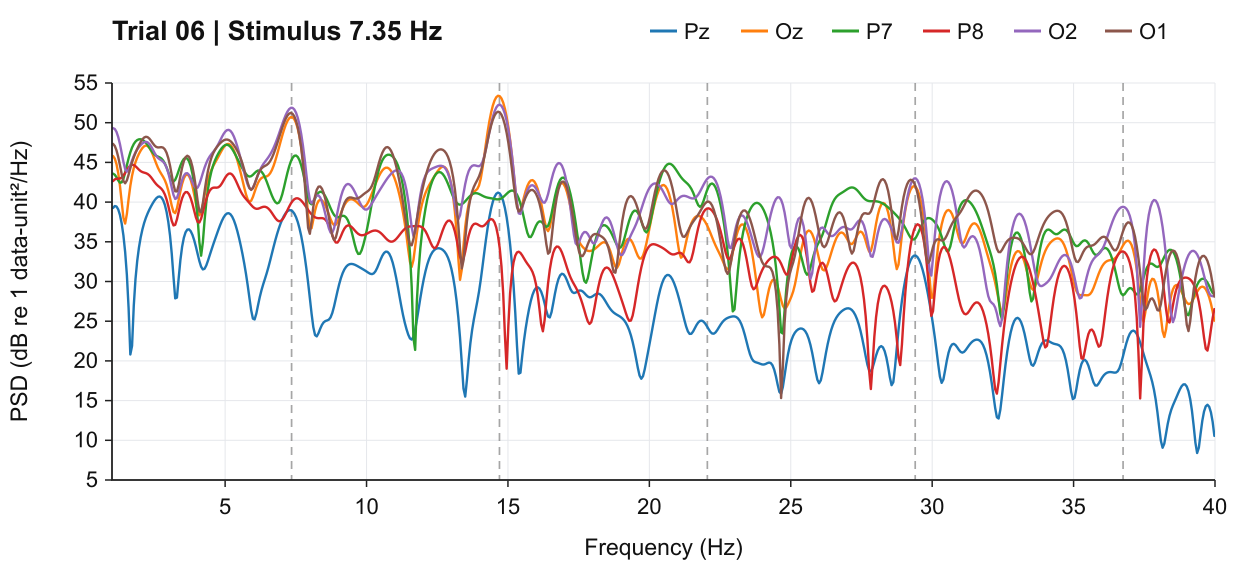
\includegraphics[width=0.9\textwidth,height=0.4\textheight,keepaspectratio]{fig20_ssvep_trial06_7p35hz.png}
\caption{Repetition 6 with a stimulation frequency of 7.35~Hz; all six channels are shown on one axis.}
\label{fig:app20}
\end{figure}

\begin{figure}[p]
\centering
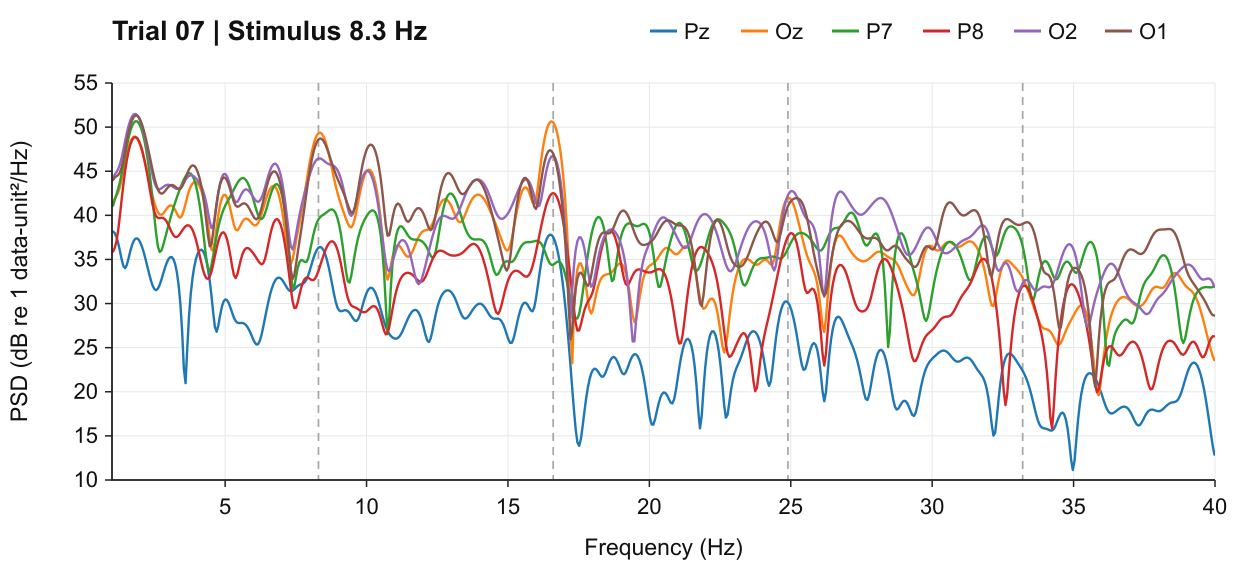
\includegraphics[width=0.9\textwidth,height=0.4\textheight,keepaspectratio]{fig21_ssvep_trial07_8p3hz.png}
\caption{Repetition 7 with a stimulation frequency of 8.3~Hz; all six channels are shown on one axis.}
\label{fig:app21}
\end{figure}

\begin{figure}[p]
\centering
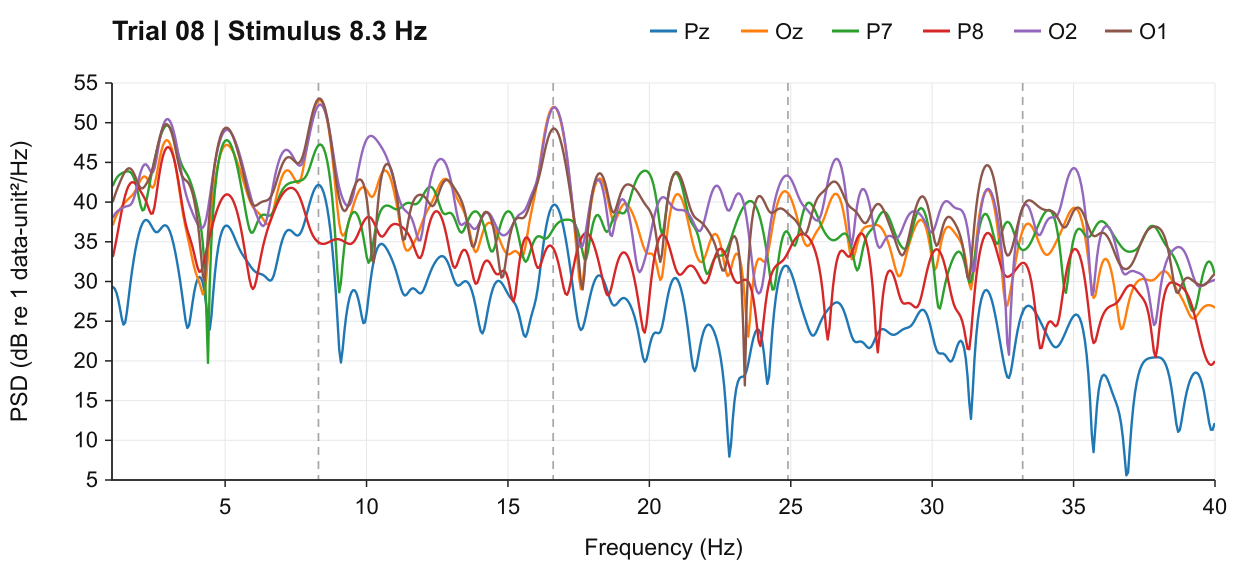
\includegraphics[width=0.9\textwidth,height=0.4\textheight,keepaspectratio]{fig22_ssvep_trial08_8p3hz.png}
\caption{Repetition 8 with a stimulation frequency of 8.3~Hz; all six channels are shown on one axis.}
\label{fig:app22}
\end{figure}

\begin{figure}[p]
\centering
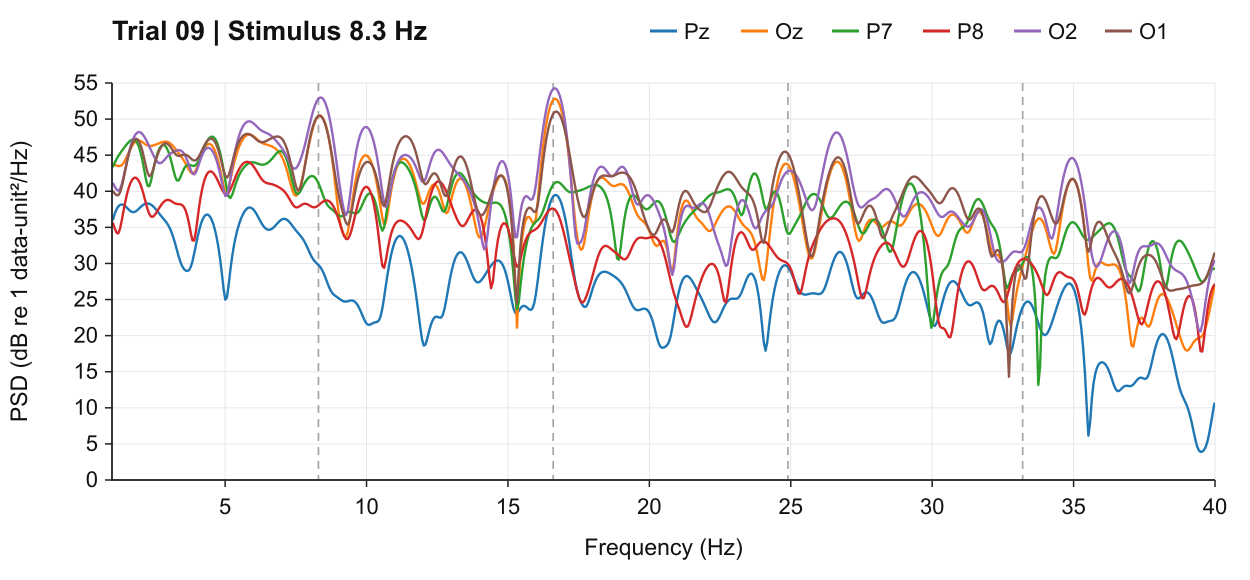
\includegraphics[width=0.9\textwidth,height=0.4\textheight,keepaspectratio]{fig23_ssvep_trial09_8p3hz.png}
\caption{Repetition 9 with a stimulation frequency of 8.3~Hz; all six channels are shown on one axis.}
\label{fig:app23}
\end{figure}

\begin{figure}[p]
\centering
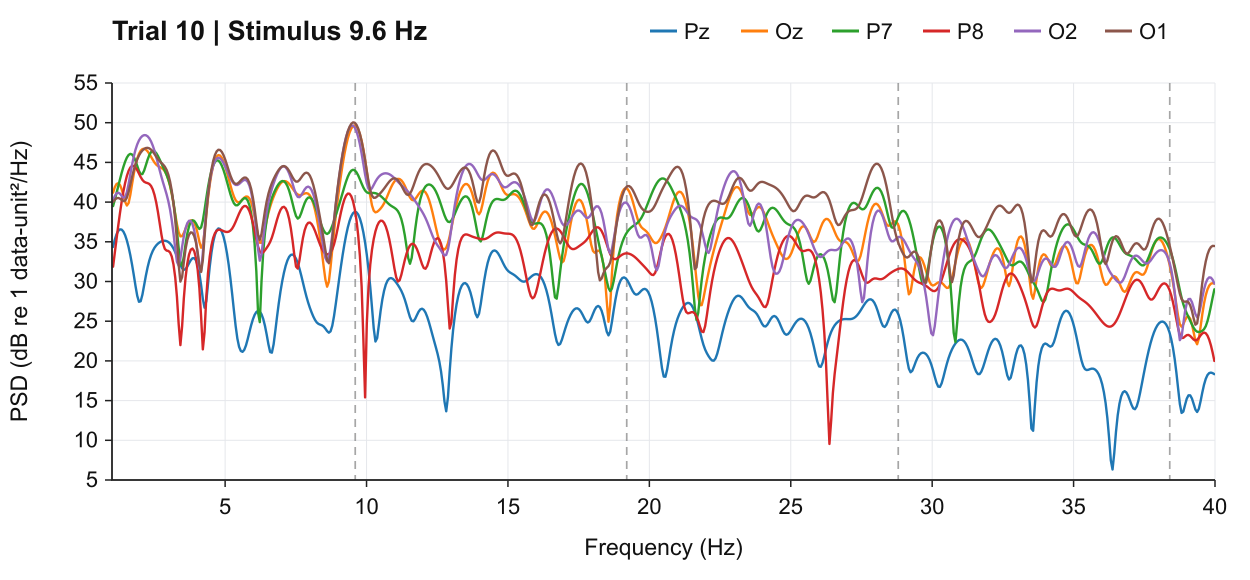
\includegraphics[width=0.9\textwidth,height=0.4\textheight,keepaspectratio]{fig24_ssvep_trial10_9p6hz.png}
\caption{Repetition 10 with a stimulation frequency of 9.6~Hz; all six channels are shown on one axis.}
\label{fig:app24}
\end{figure}

\begin{figure}[p]
\centering
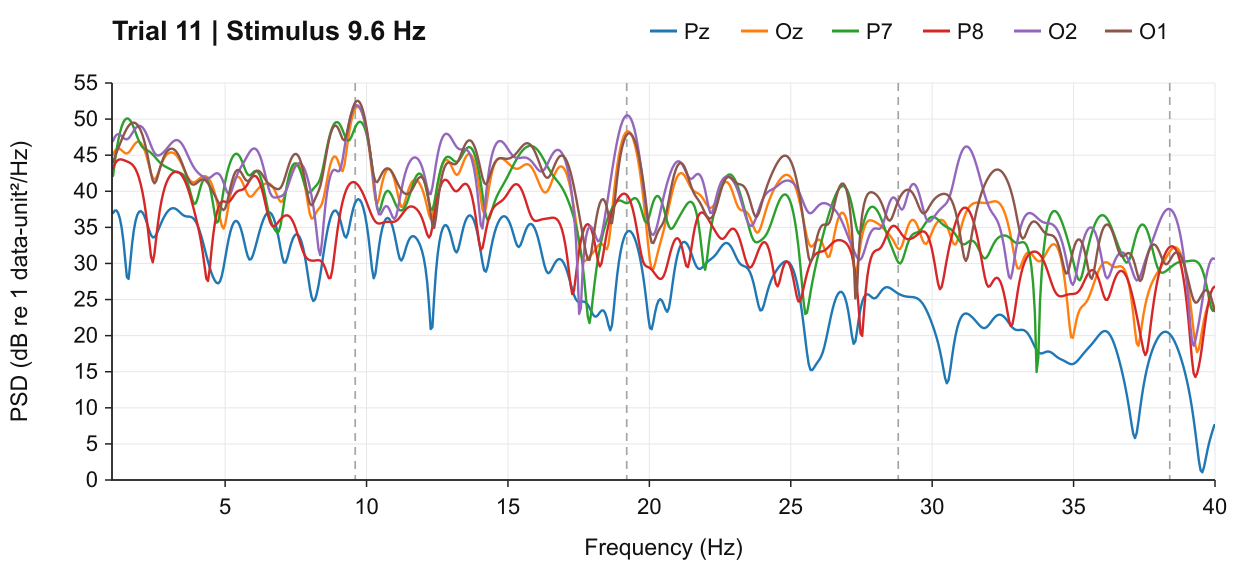
\includegraphics[width=0.9\textwidth,height=0.4\textheight,keepaspectratio]{fig25_ssvep_trial11_9p6hz.png}
\caption{Repetition 11 with a stimulation frequency of 9.6~Hz; all six channels are shown on one axis.}
\label{fig:app25}
\end{figure}

\begin{figure}[p]
\centering
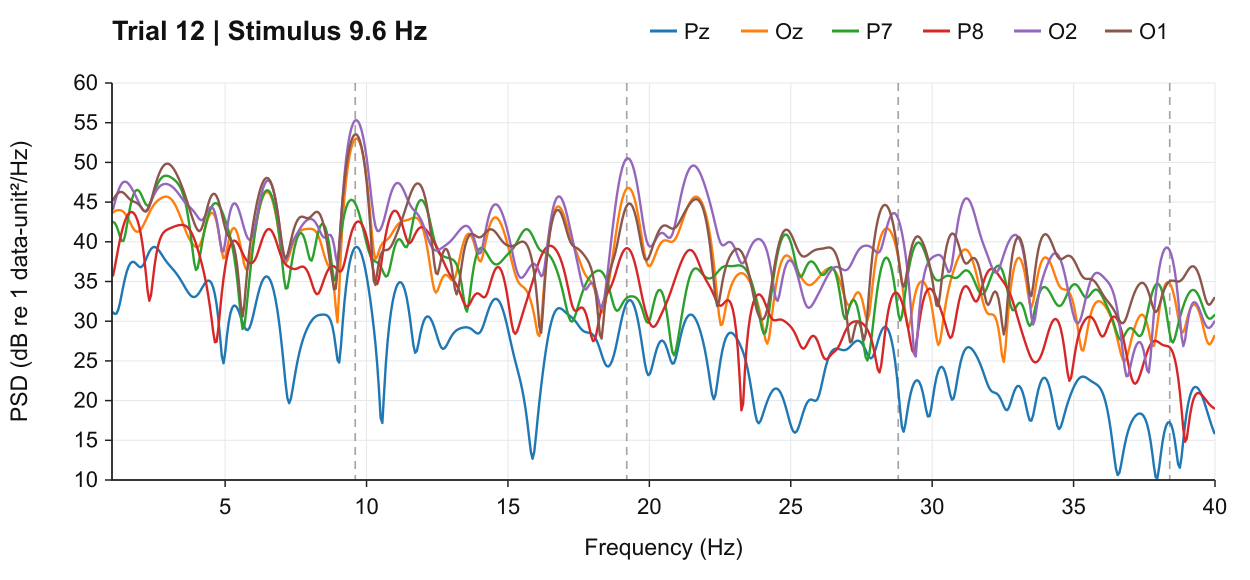
\includegraphics[width=0.9\textwidth,height=0.4\textheight,keepaspectratio]{fig26_ssvep_trial12_9p6hz.png}
\caption{Repetition 12 with a stimulation frequency of 9.6~Hz; all six channels are shown on one axis.}
\label{fig:app26}
\end{figure}

\begin{figure}[p]
\centering
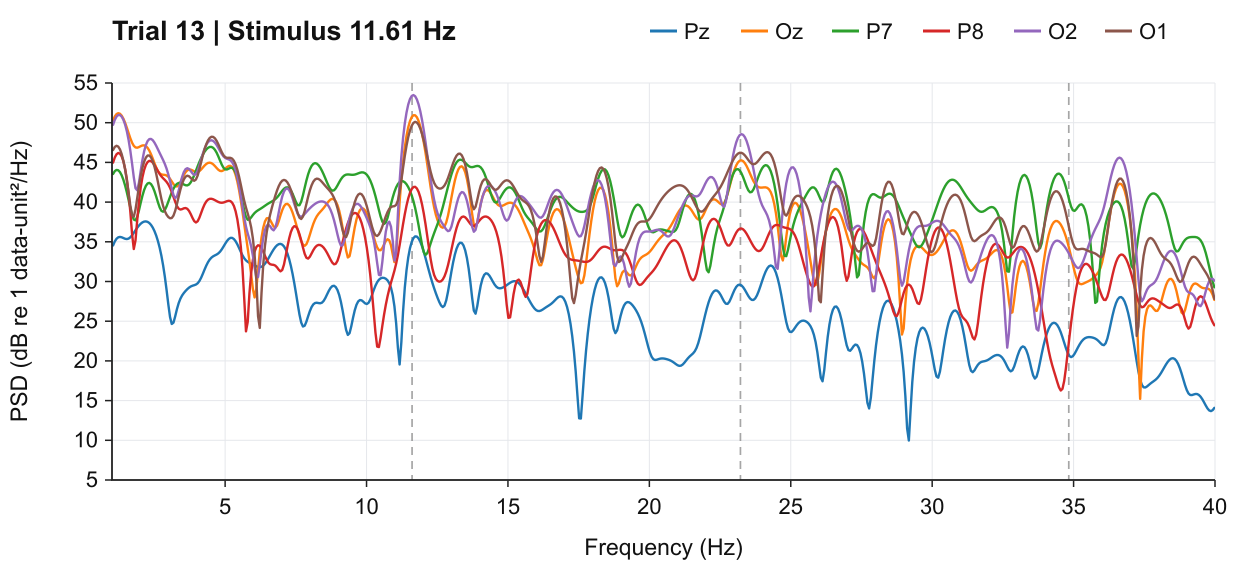
\includegraphics[width=0.9\textwidth,height=0.4\textheight,keepaspectratio]{fig27_ssvep_trial13_11p61hz.png}
\caption{Repetition 13 with a stimulation frequency of 11.61~Hz; all six channels are shown on one axis.}
\label{fig:app27}
\end{figure}

\begin{figure}[p]
\centering
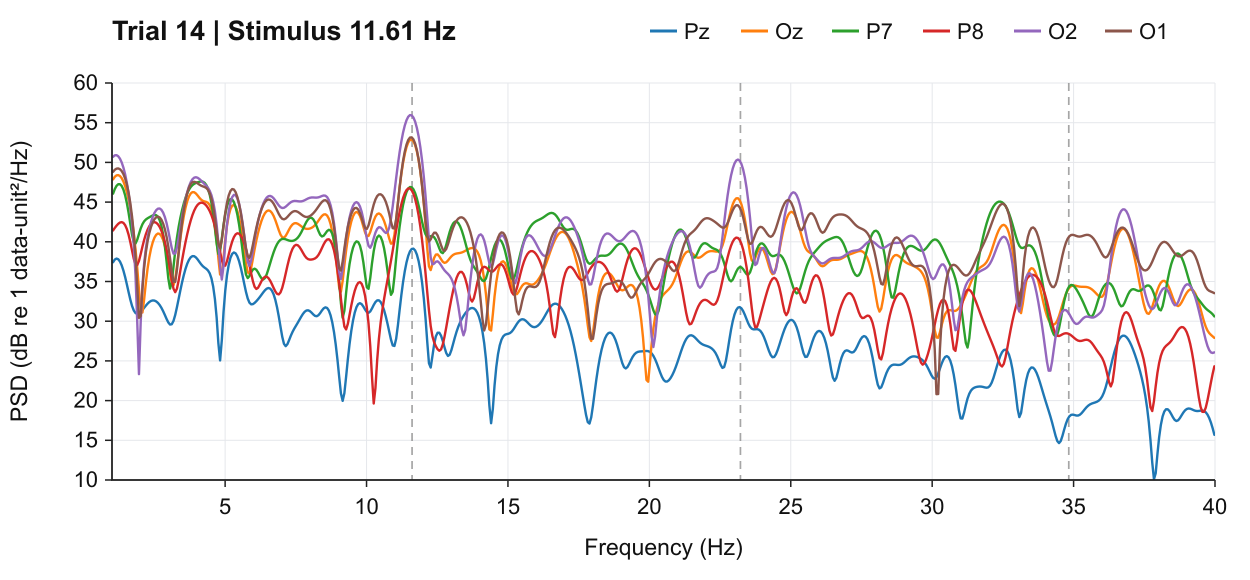
\includegraphics[width=0.9\textwidth,height=0.4\textheight,keepaspectratio]{fig28_ssvep_trial14_11p61hz.png}
\caption{Repetition 14 with a stimulation frequency of 11.61~Hz; all six channels are shown on one axis.}
\label{fig:app28}
\end{figure}

\begin{figure}[p]
\centering
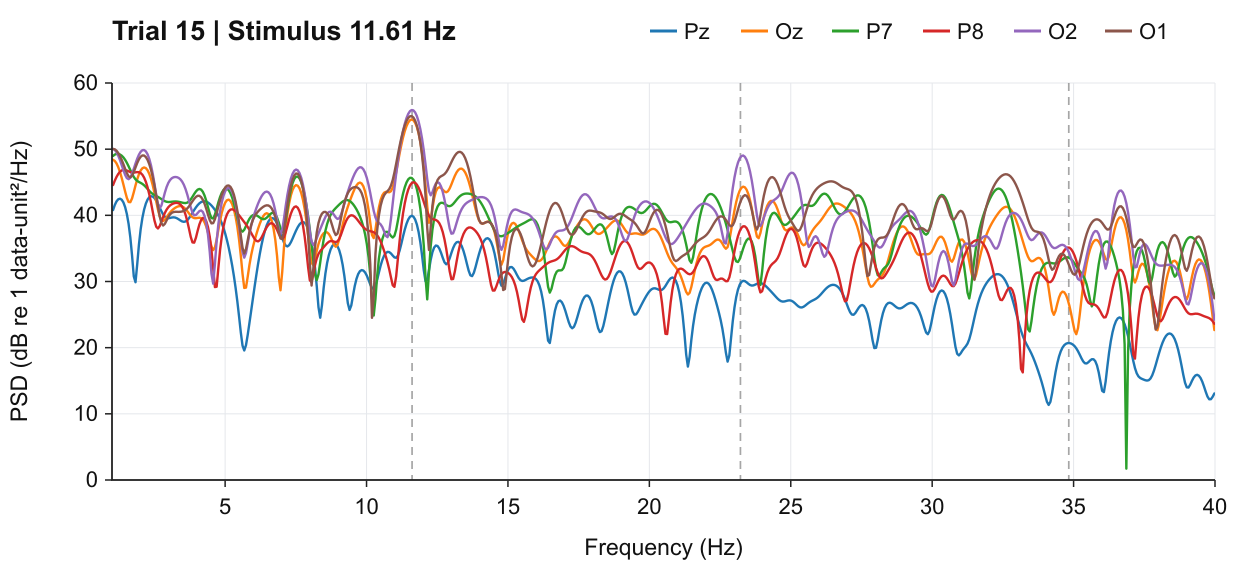
\includegraphics[width=0.9\textwidth,height=0.4\textheight,keepaspectratio]{fig29_ssvep_trial15_11p61hz.png}
\caption{Repetition 15 with a stimulation frequency of 11.61~Hz; all six channels are shown on one axis.}
\label{fig:app29}
\end{figure}

\begin{figure}[p]
\centering
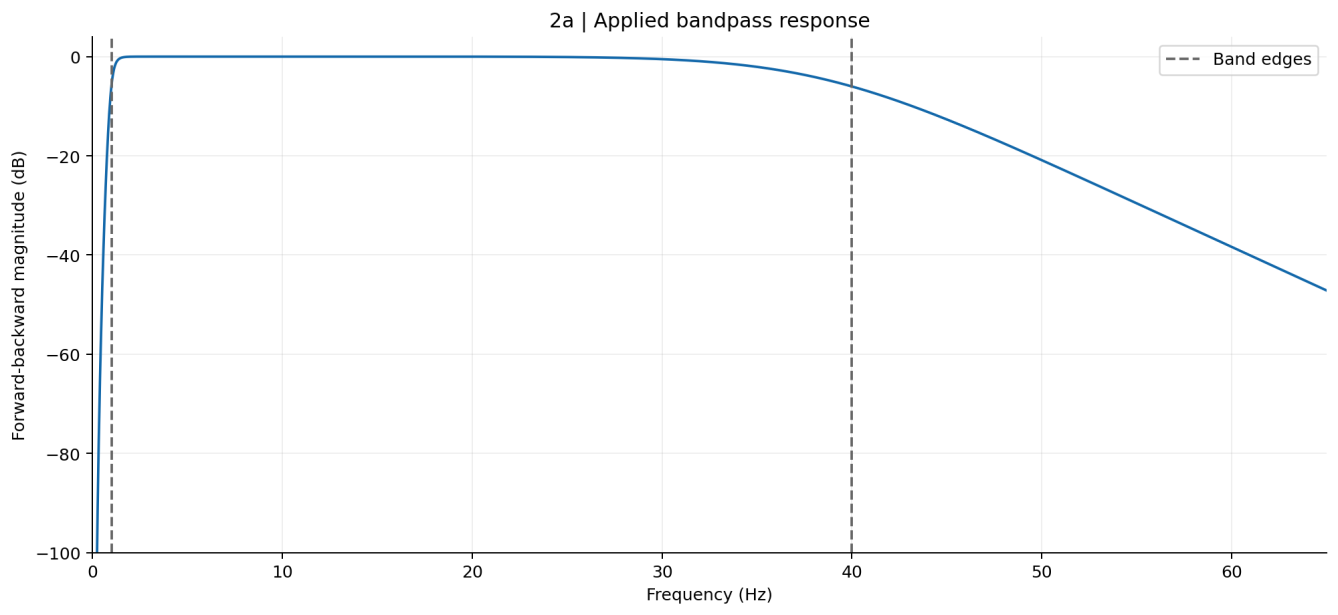
\includegraphics[width=0.9\textwidth,height=0.4\textheight,keepaspectratio]{fig30_zero_phase_filter_response.png}
\caption{Amplitude response of the forward--backward filter applied in Part~2; the transition on the two sides of the band is gradual.}
\label{fig:app30}
\end{figure}
